\documentclass[12pt]{article}
\usepackage[a4paper, margin=2cm]{geometry}
\usepackage[english]{babel} % To obtain English text with the blindtext package
\usepackage{blindtext}
\usepackage{graphicx} % Required for inserting images
\usepackage{array, multirow} % For extra column formatting
\usepackage{amsmath, amssymb, cancel} %for equation environment
\usepackage{float}
\usepackage{parskip} % For gaps between para
\usepackage{setspace}
\usepackage{pdfpages}
\usepackage{abstract}
\usepackage[export]{adjustbox}
\usepackage{emptypage}
\usepackage{tocloft}
\usepackage[nottoc]{tocbibind}
\usepackage{hyperref, url}
\usepackage[table]{xcolor}
\usepackage{minted}
    \usemintedstyle{monokai}
\usepackage{caption}
    \captionsetup{font=footnotesize,labelfont=bf}
\usepackage{tcolorbox}
    \newtcolorbox{mintedbox}{
        colback=backcolour,
        boxrule=0pt,
        sharp corners,
        width=\linewidth,
        left=0pt, right=0pt,
        top=3pt, bottom=3pt
    }

\cftsetindents{section}{0em}{2em}
\cftsetindents{subsection}{0em}{2em}

\renewcommand\cfttoctitlefont{\hfill\Large\bfseries}
\renewcommand\cftaftertoctitle{\hfill\mbox{}}

\graphicspath{ {./images/} }

\pagenumbering{arabic}

\definecolor{blurple}{HTML}{5865F2}
\definecolor{backcolour}{HTML}{272823}

\hypersetup{
    colorlinks=true,
    linkcolor=black,
    urlcolor=blurple,
    citecolor=blurple,
}

\urlstyle{same}

\renewcommand{\arraystretch}{1.3}

\setcounter{secnumdepth}{5}
\setcounter{tocdepth}{5}
\newcommand\simpleparagraph[1]{%
  \stepcounter{paragraph}\paragraph*{\theparagraph\quad{}#1}}

%%%%%%%%%%%%%%%%%%%%%%%%%%%%%%%%%%%


\title{PHYC20040 Exp.2 Pleiades SM}
\author{Joana Adao}
\date{\today}

\begin{document}

\begin{titlepage}
    \begin{center}

        \begin{figure}[ht]
            
\includegraphics[width=\textwidth]{UCDLogo.png}
        \end{figure}
        
        \begin{figure}
            \centerline{
\includegraphics[width=\paperwidth]{UCDBanner.png}}
        \end{figure}

        \vspace{4cm}

        {\LARGE \bfseries PHYC20080 Fields, Waves and Light}\\
        \vspace{0.75cm}
        {\Large Experiment No.2 Waves and Resonance}
        
        \vspace{1cm}
    
    {\Large \textbf{18 February 2025}}

    \vspace{2cm}
    
    {\large \textbf{by Joana C.C. Adao (Student No. 23311051)}}\\
    \vspace{.25cm}
    {\large \textbf{With,} Beau Etac}\\
    \vspace{0.25cm}
    {\large Tuesday 16.00-18.00 Slot}\\
    {\large Nicki (Coordinator)}

    \end{center}
    
   \clearpage

\end{titlepage}

\setcounter{page}{1}
\tableofcontents

\newpage

\begin{abstract}
\addcontentsline{toc}{section}{Abstract}

The aim of this experiment was to find the resonant of a stretched string when varying the length and tension across it individually.
Frequency was varied with the use of an oscillator and the resonant frequencies were recorded. The frequency was plotted against the inverse of the length of the string, and
a separate graph for the square of the frequency against the tension across the string was plotted as well.

The percentage difference between both the theoretical (\textbf{22.327}) and calculated (\textbf{0.0294}) slope is found to be \textbf{199.47\%} for the inverse length relationship, which is an incredibly significant difference.
The percentage difference between both the theoretical (\textbf{1 780.627}) and calculated (\textbf{13 542.891}) slope is found to be \textbf{153.52\%} for the tension relationship, which is also an incredibly significant difference.

\end{abstract}

%%%%%%%%%%%%%%%%%%%%%%%%%%%%%%%%%%%

\vspace{3.5cm}
\section{Theory} \label{sec:1}


\subsection{Waves}

There are two types of mechanical waves, as illustrated in figure \ref{fig:wavetype}, \textbf{transverse} and \textbf{longitudinal}.

\begin{minipage}{.47\textwidth}
    \captionsetup{hypcap=false}
    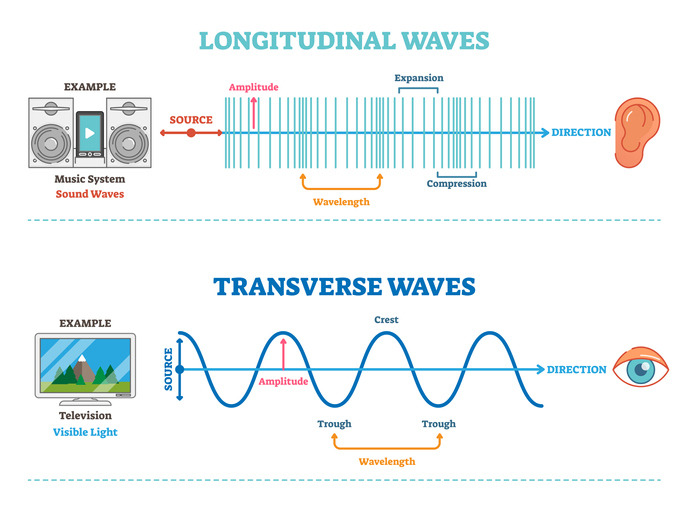
\includegraphics[width=\linewidth]{wavetype.jpg}
    \captionof{figure}{\centering Types of waves \protect\cite{waveoer}.}
    \label{fig:wavetype}
\end{minipage}
\hfill
\begin{minipage}{.51\textwidth}
    \captionsetup{hypcap=false}
    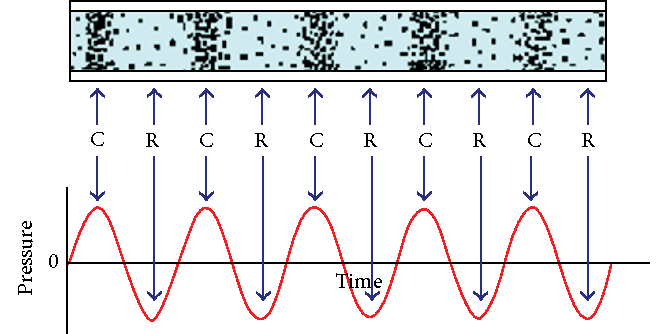
\includegraphics[width=\linewidth]{longtrans.png}
    \captionof{figure}{\centering Longitudinal wave graphed as a transverse wave \protect\cite{mungwave}.}
    \label{fig:longtrans}
\end{minipage}

\textbf{Transverse waves} travel in a series of peaks and troughs with \textit{perpendicular} vibration to the motion. These are the kinds of waves seen when water ripples \cite{waveffden}.
\textbf{Longitudinal waves} vibrate \textit{parallel} to the motion. Instead of peaks and troughs there are areas of compression, in which the molecules around it bunch together, and
areas of rarefraction, in which the molecules are pulled away and space out \cite{waveffden,studywave,acousticsound}.
Through graphing, a longitudinal wave can appear as a transverse wave where the peaks represent compression and troughs represent rarefraction (see figure \ref{fig:longtrans}).

\newpage
\subsubsection{The Anatomy of a Wave}

There are 4 basic components to a wave \cite{wavebyju,waveffden}, with all components illustrated in figure \ref{fig:waveprop}:

\begin{itemize}
    \item \textbf{Frequency (f):} the number of waves that pass by a point per second (repetitions).
    \item \textbf{Period (T):} time taken for a wave to pass a specific point in a second.
    \item \textbf{Wavelength ($\mathbf{\lambda}$):} the distance between two waves, crest (peak) to crest or trough (valley) to trough.
    \item \textbf{Amplitude (A):} the 'height' of the wave measured from the middle (x-axis) of the wave to the crest/trough.
\end{itemize}

\begin{figure}[H]
    \centering
    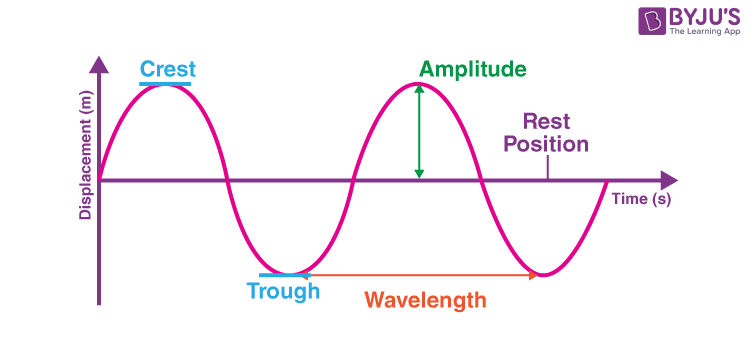
\includegraphics[width=14cm]{wave.png}
    \caption{\centering Features of a wave \protect\cite{wavebyju}}
    \label{fig:waveprop}
\end{figure}


\subsubsection{Newton's Laws and Wave Velocity}

The velocity of a wave can be found at a specific point on a waveform (a point of fixed phase) by relating the wavelength to the period/frequency \cite{geekwave,librewave}:

\vspace{-1.5ex}
\begin{gather} \label{eq:1}
    v = \frac{\lambda}{T} = \lambda f
\end{gather}

Furthermore, by applying Newton's second law to the vertical direction of the wave the following is able to be derived \cite{librewave}:

\vspace{-1.5ex}
\begin{gather} \label{eq:2}
    v = \sqrt{\frac{\textbf{F}}{\mu}} = \sqrt{\frac{T}{\mu}}
\end{gather}

Where \textbf{F} is a force acting on the wave, pulling through the string. This can be defined as the tension \textbf{T}, the force of a stretched material (eg. string). $\mathbf{\mu}$ is then
the mass per unit length of the string.

\subsection{Resonance}

Resonance is a phenomenon in which an object will vibrate more strongly when an external oscillation that matches its own natural frequency passes through it \cite{resbrit,reslibre}.

Equation \ref{eq:1} and equation \ref{eq:1} can be combined to give the following:

\vspace{-1.5ex}
\begin{gather} \label{eq:3}
    \lambda f = \sqrt{\frac{T}{\mu}} \quad \implies \quad f = \frac{1}{\lambda} \sqrt{\frac{T}{\mu}}
\end{gather}

\subsubsection{Standing Waves} \label{sec:1.2.1}

Standing waves are produced as a result of interference from the \textit{reflected wave} when a wave encounters a boundary between two mediums \cite{librestand,MARION1981341,OZEROV2007105,isaacwave}.
There appears to be a point along the axis of the wave which is fixed and the wave oscillates on, known as \textit{nodes}. The rest of the wave that moves to the crests and troughs are known as \textit{antinodes}
\cite{isaacwave}.
The resulting wave is a superposition of the adjacent nodes and antinodes that are, naturally, in phase \cite{isaacwave,librestand,MARION1981341}.

\begin{figure}[H]
    \centering
    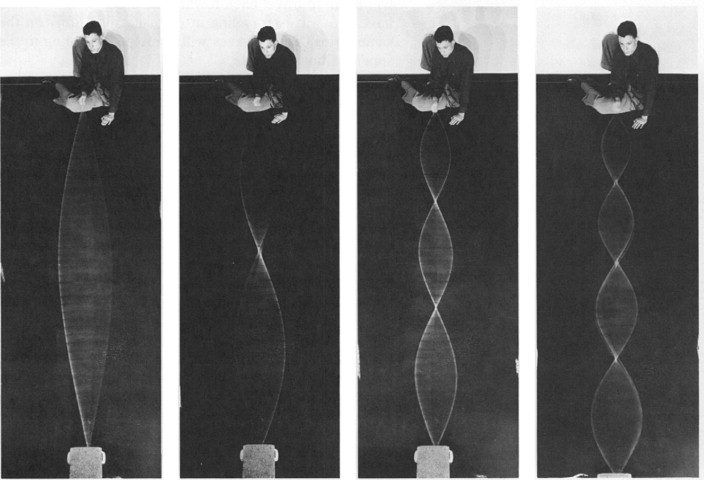
\includegraphics[width=10cm]{standing waves.jpg}
    \caption{\centering Standing waves in a stretched rubber tube \protect\cite{MARION1981341}.}
    \label{fig:stand}
\end{figure}

The lowest frequency at which a standing wave only produces a wave pattern at the nodes on the fixed ends is known as the \textbf{fundamental frequency} and can
be observed in the far left image of figure \ref{fig:stand}.

This frequency is represented by the following \cite{isaacwave,librestand,MARION1981341}, with \textbf{L} as the length, \textbf{n} as the $n^{th}$ multiple of the funcamental harmonic (see §\ref{sec:1.2.2}), and $\mathbf{\lambda_n}$ as
the frequency at the $n^{th}$ harmonic:

\vspace{-1.5ex}
\begin{gather} \label{eq:4}
    \lambda_n = \frac{2L}{n}
\end{gather}

This equation can then be applied to equation \ref{eq:3} to obtain the following for the resonant frequency:

\vspace{-1.5ex}
\begin{gather} \label{eq:5}
    f_{resonant} = \frac{n}{2L} \sqrt{\frac{T}{\mu}}
\end{gather}

\subsubsection{Harmonics} \label{sec:1.2.2}

Harmonics of a standing wave are as discussed in §\ref{sec:1.2.1}, positive interger multiples of the first harmonic, also known as the fundamental frequency, at which the 
standing wave oscillates at. In figure \ref{fig:stand} the second, third and fourth harmonics of the standing wave can be seen (left to right) \cite{MARION1981341}.

\begin{table}[H]
    \centering
    \caption{\centering Table of a summary of the harmonic relationships \protect\cite{classharmonicsm}.}
    \begin{tabular}{c|c|c|c|c}
    \textbf{\begin{tabular}[c]{@{}c@{}}Harmonic\\ \#\end{tabular}} &
      \textbf{\begin{tabular}[c]{@{}c@{}}\# of Waves\\ in String\end{tabular}} &
      \textbf{\begin{tabular}[c]{@{}c@{}}\# of \\ Nodes\end{tabular}} &
      \textbf{\begin{tabular}[c]{@{}c@{}}\# of\\ Anti-nodes\end{tabular}} &
      \textbf{\begin{tabular}[c]{@{}c@{}}Length-Wavelength\\ Relationship\end{tabular}} \\
    \textbf{1} & 1/2     & 2 & 1 & $\lambda = 2L$  \\
    \textbf{2} & 1 (2/2) & 3 & 2 & $\lambda = L$            \\
    \textbf{3} & 3/2     & 4 & 3 & $\lambda = \frac{3}{2L}$ \\
    \textbf{4} & 2 (4/2) & 5 & 4 & $\lambda = \frac{2}{L}$ \\
    \textbf{5} & 5/2     & 6 & 5 & $\lambda = \frac{5}{2L}$
    \end{tabular}
\end{table}

\vspace{.5cm}
\section{Methodology} \label{sec:2}

The apparatus was shown as below in figure \ref{fig:appillust} for both parts of the experiment. The oscilloscope is seen in figure \ref{fig:oscil}, the string apparatus as in figure \ref{fig:exp},
and the power supply with teh connected oscillator shown in figure \ref{fig:box}.

\begin{figure}[H]
    \centering
    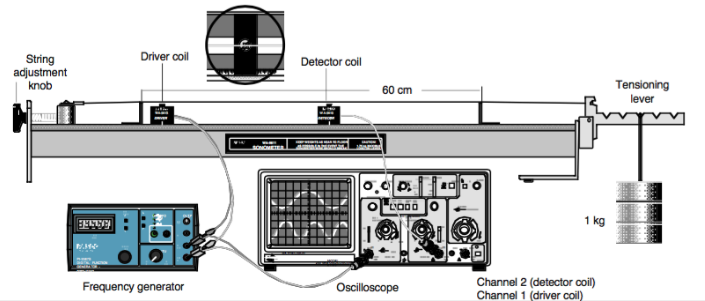
\includegraphics[width=\linewidth]{wave app.png}
    \caption{\centering Illustration of the apparatus setup \protect\cite{UCDwave}.}
    \label{fig:appillust}
\end{figure}

\begin{minipage}{.31\textwidth}
    \captionsetup{hypcap=false}
    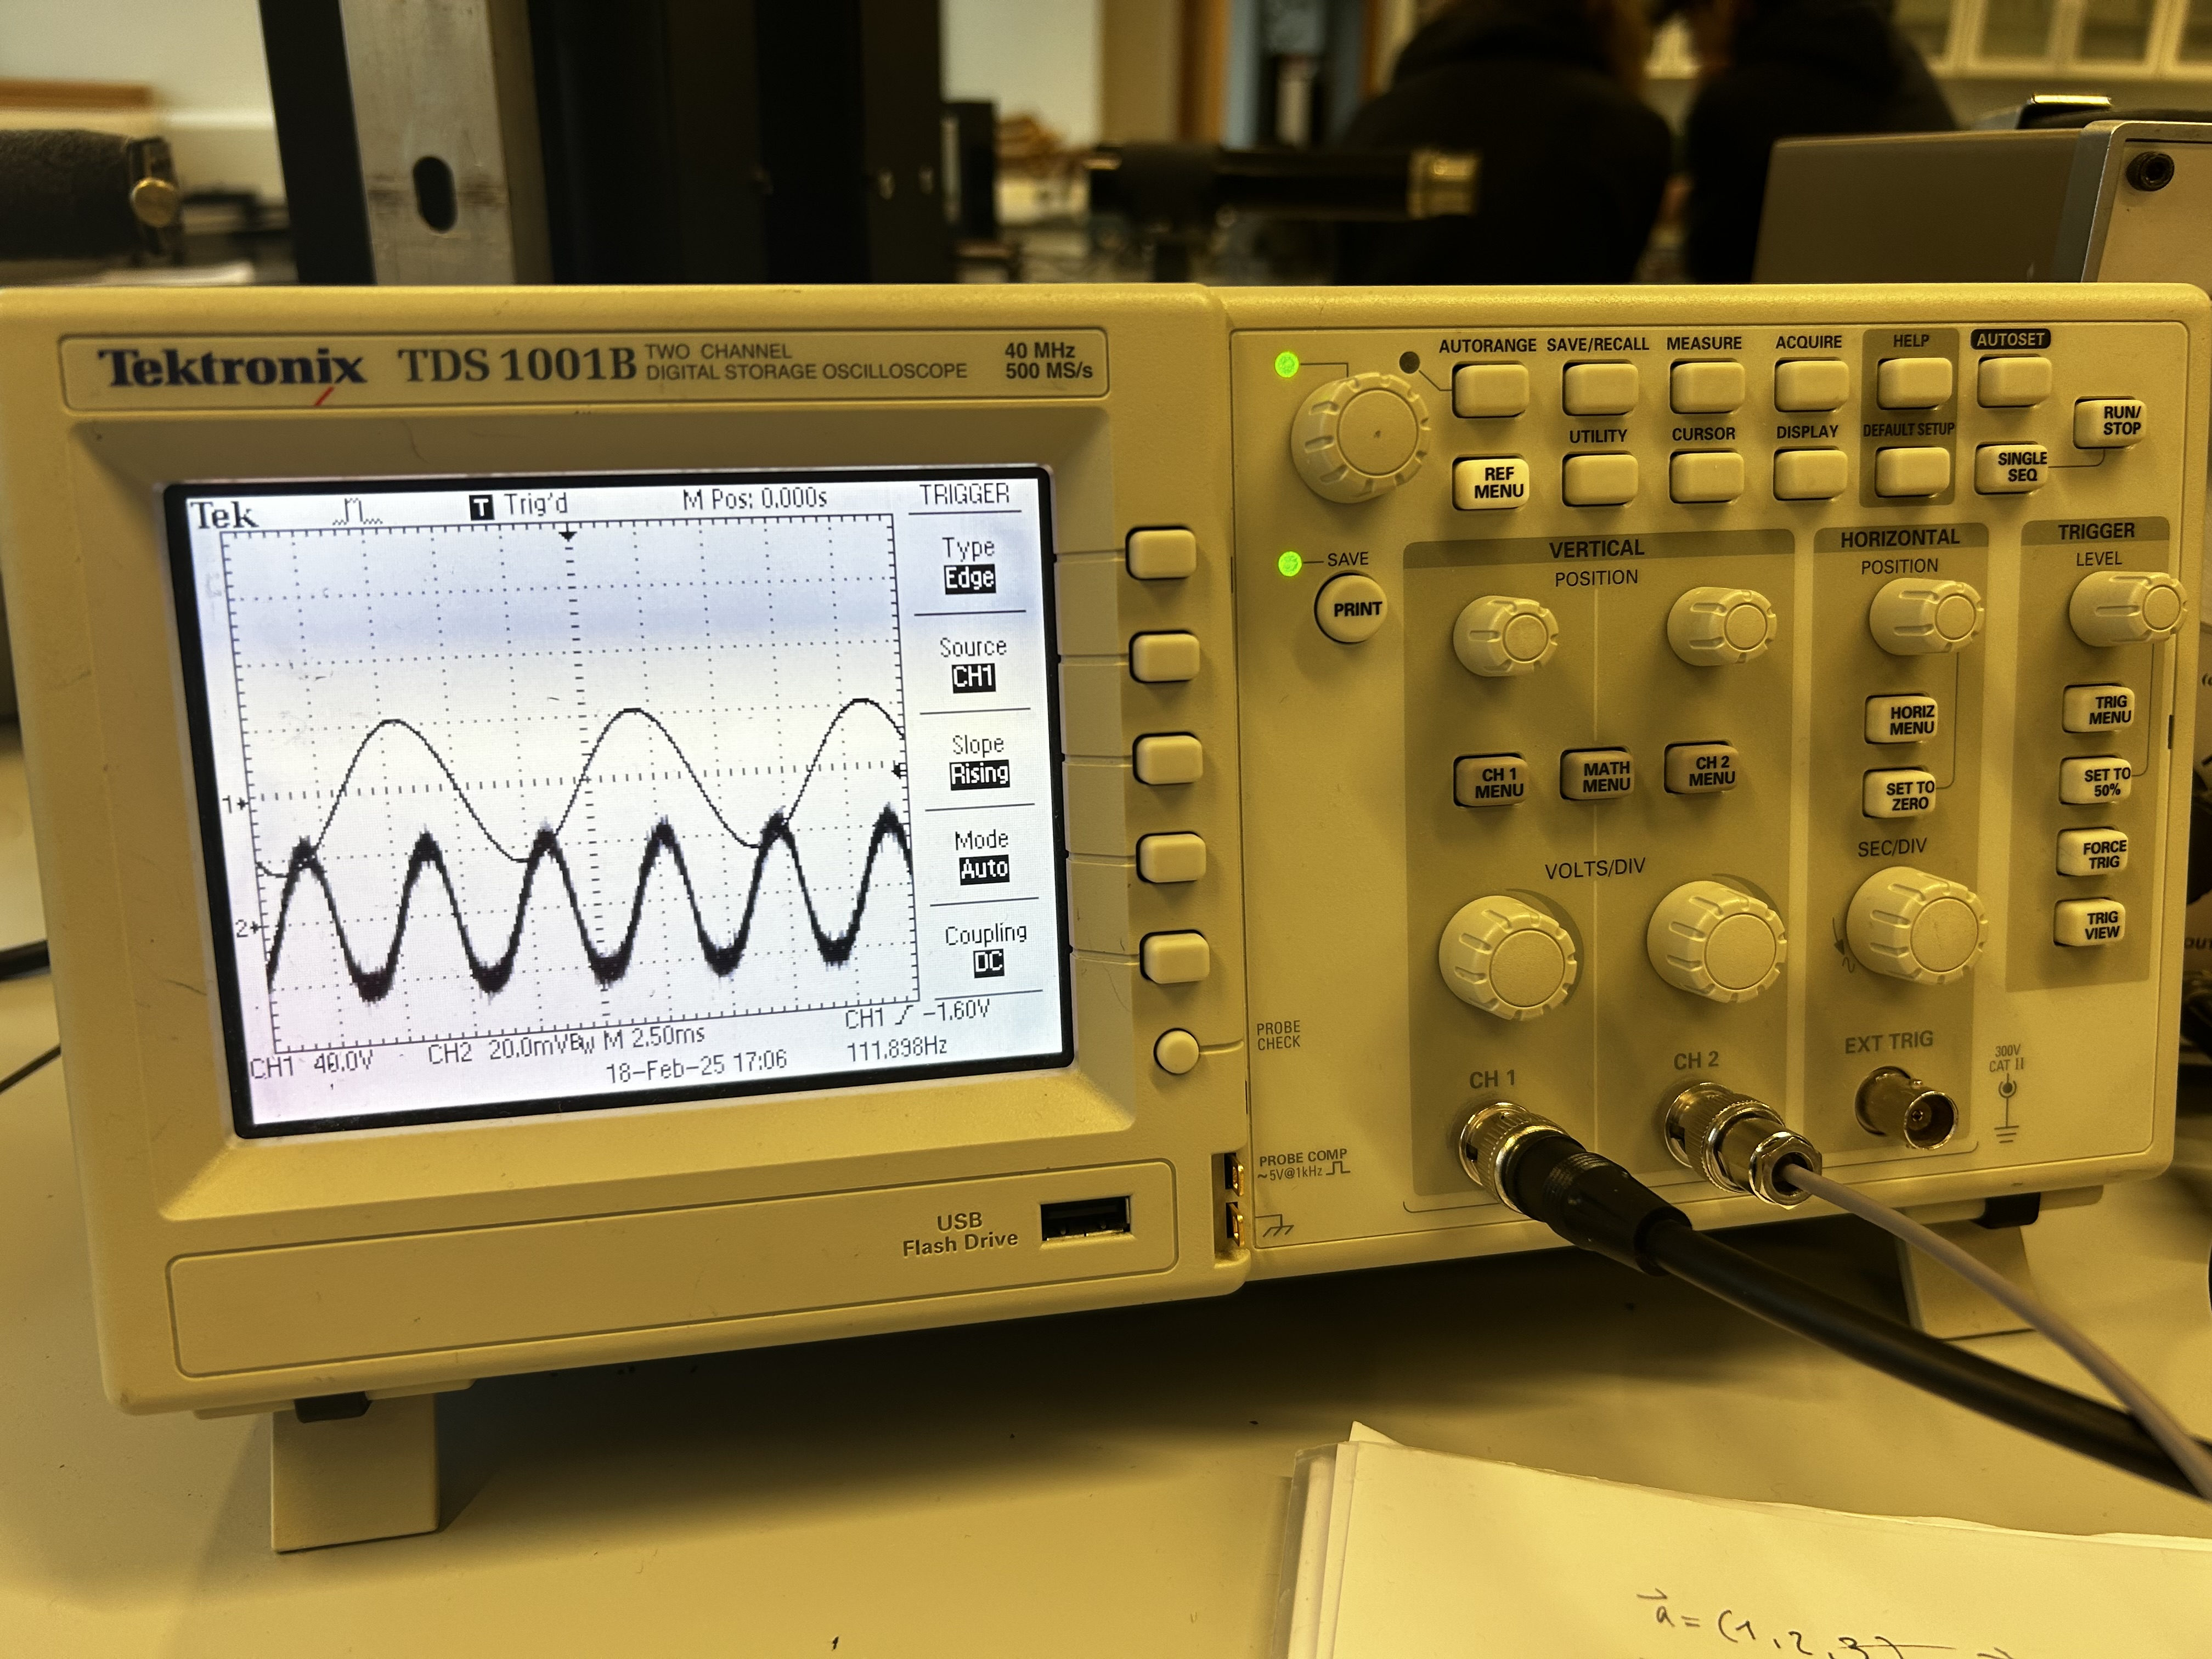
\includegraphics[width=\linewidth]{wave exp 1.jpeg}
    \captionof{figure}{\centering Image of the oscilloscope.}
    \label{fig:oscil}
\end{minipage}
\hfill
\begin{minipage}{.31\textwidth}
    \captionsetup{hypcap=false}
    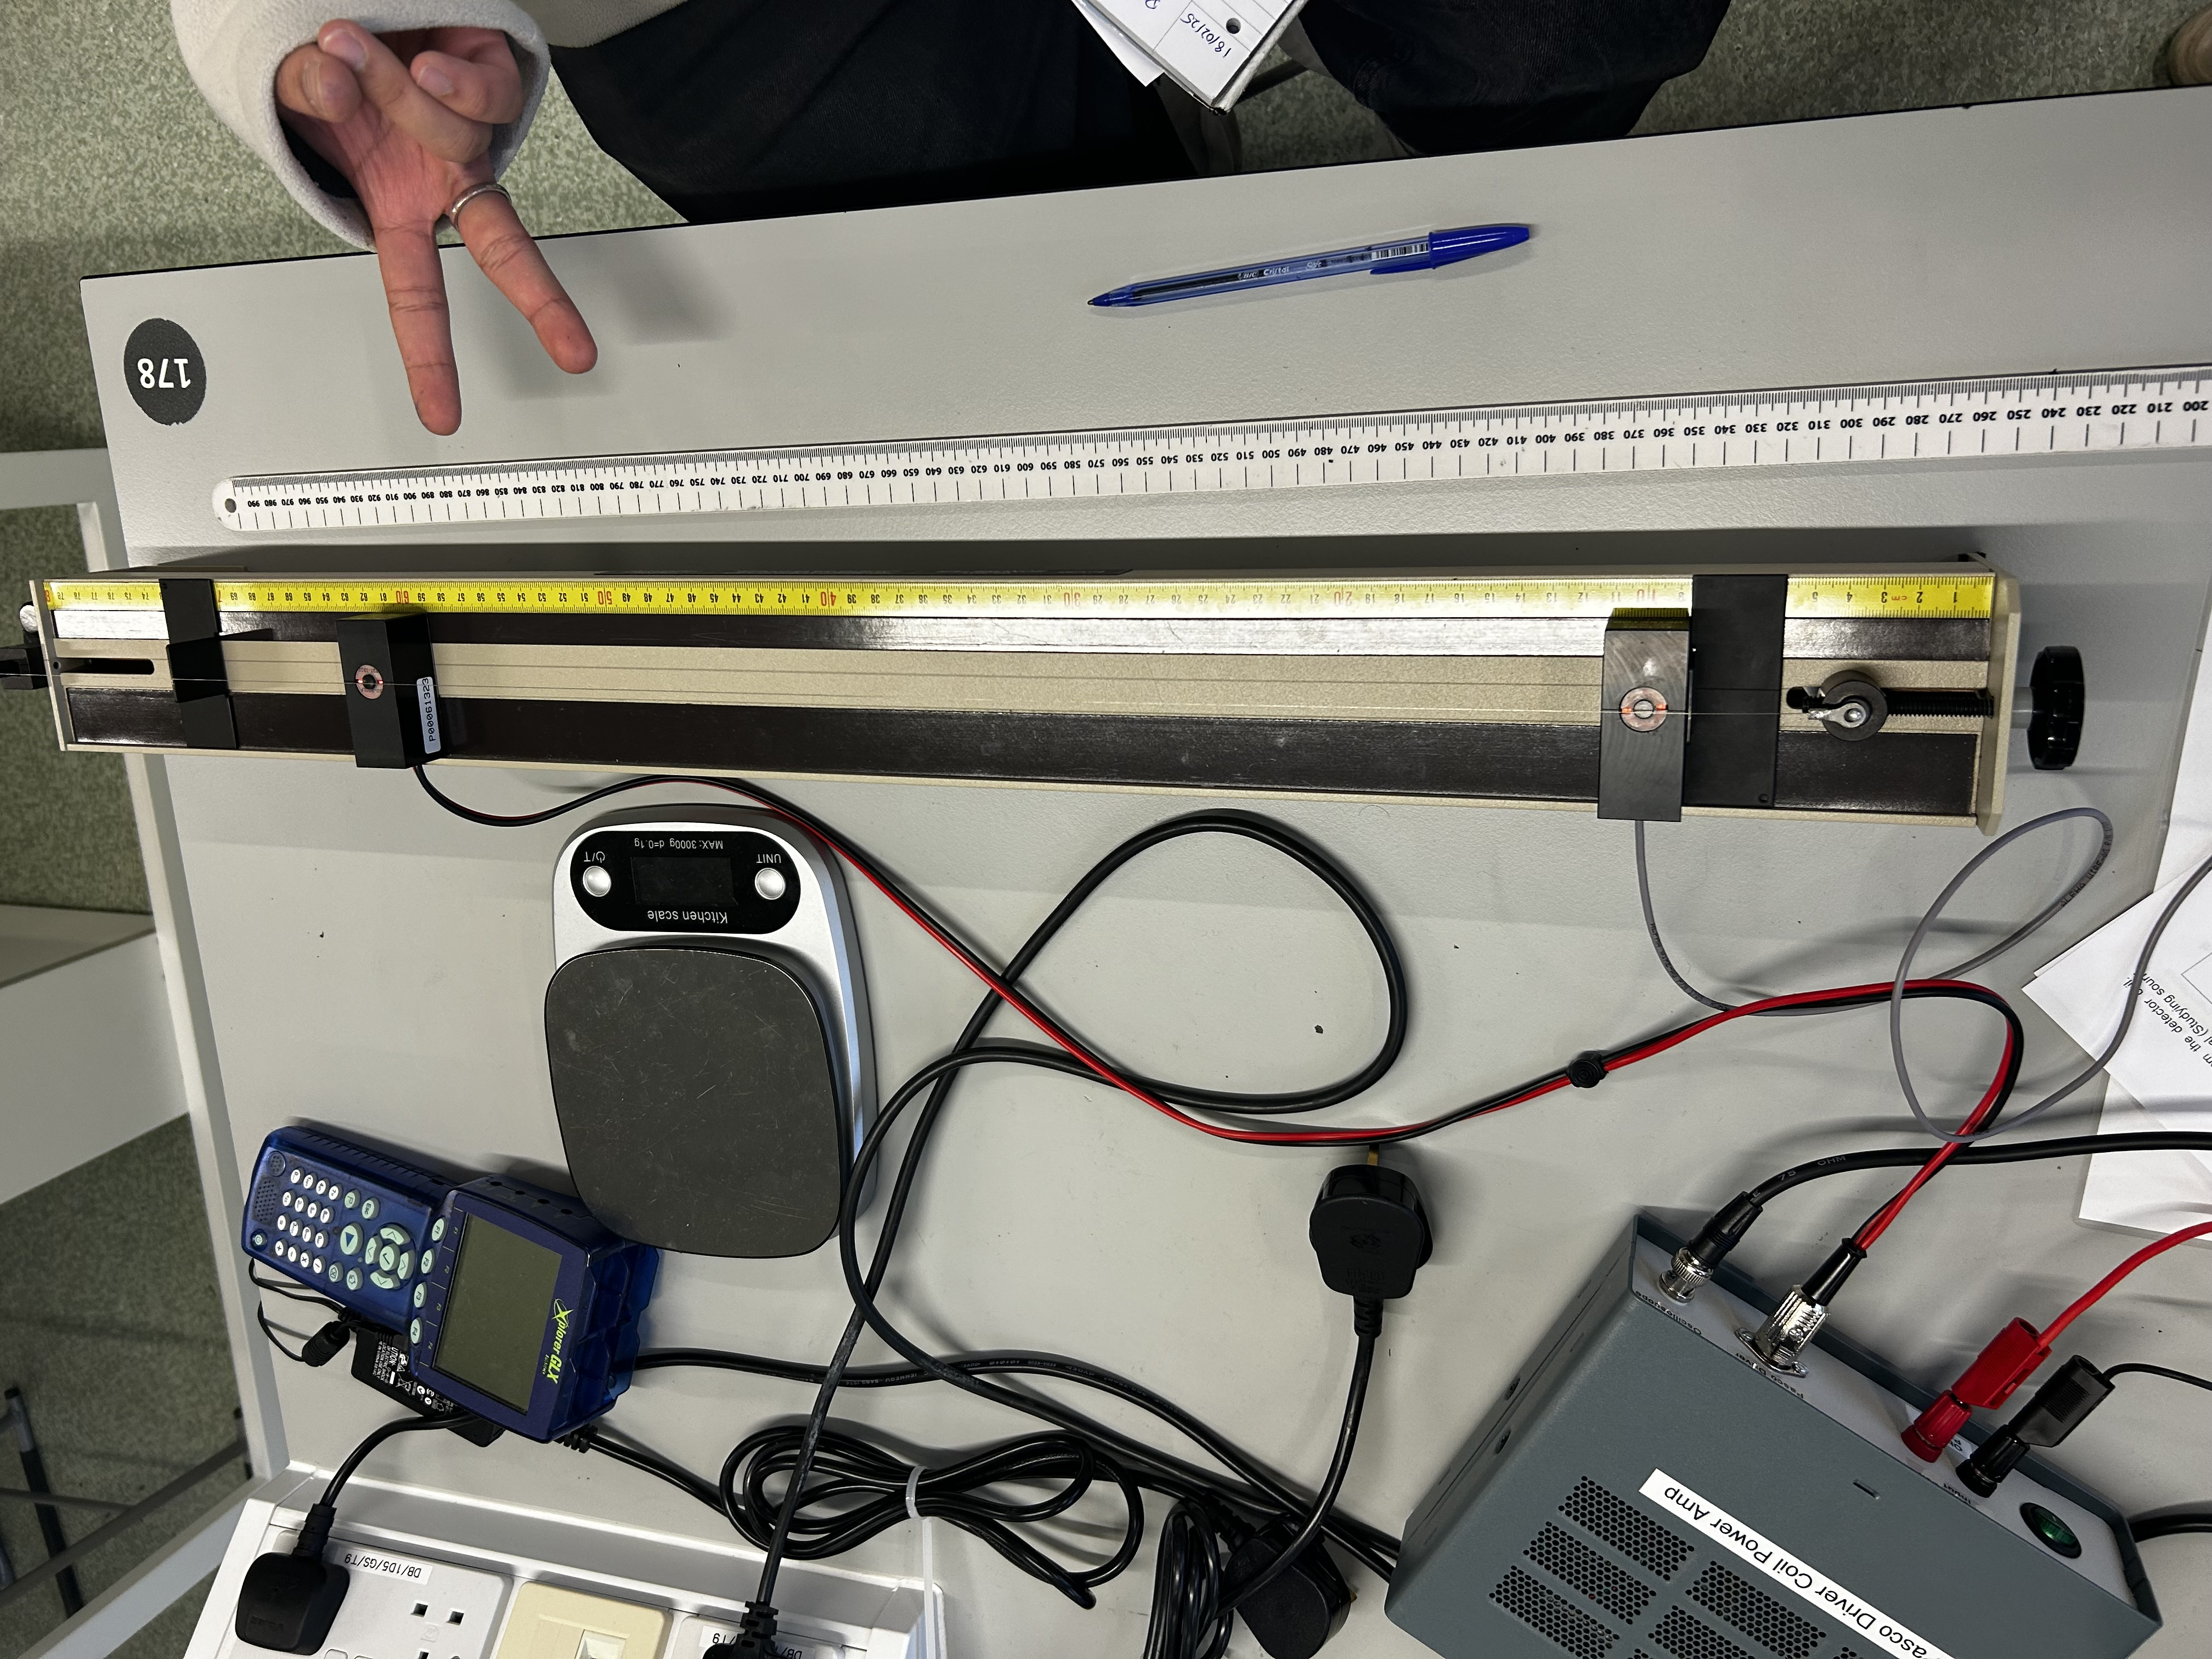
\includegraphics[width=\linewidth, angle=180]{wave exp 2.jpeg}
    \captionof{figure}{\centering Image of the experimental setup.}
    \label{fig:exp}
\end{minipage}
\hfill
\begin{minipage}{.31\textwidth}
    \captionsetup{hypcap=false}
    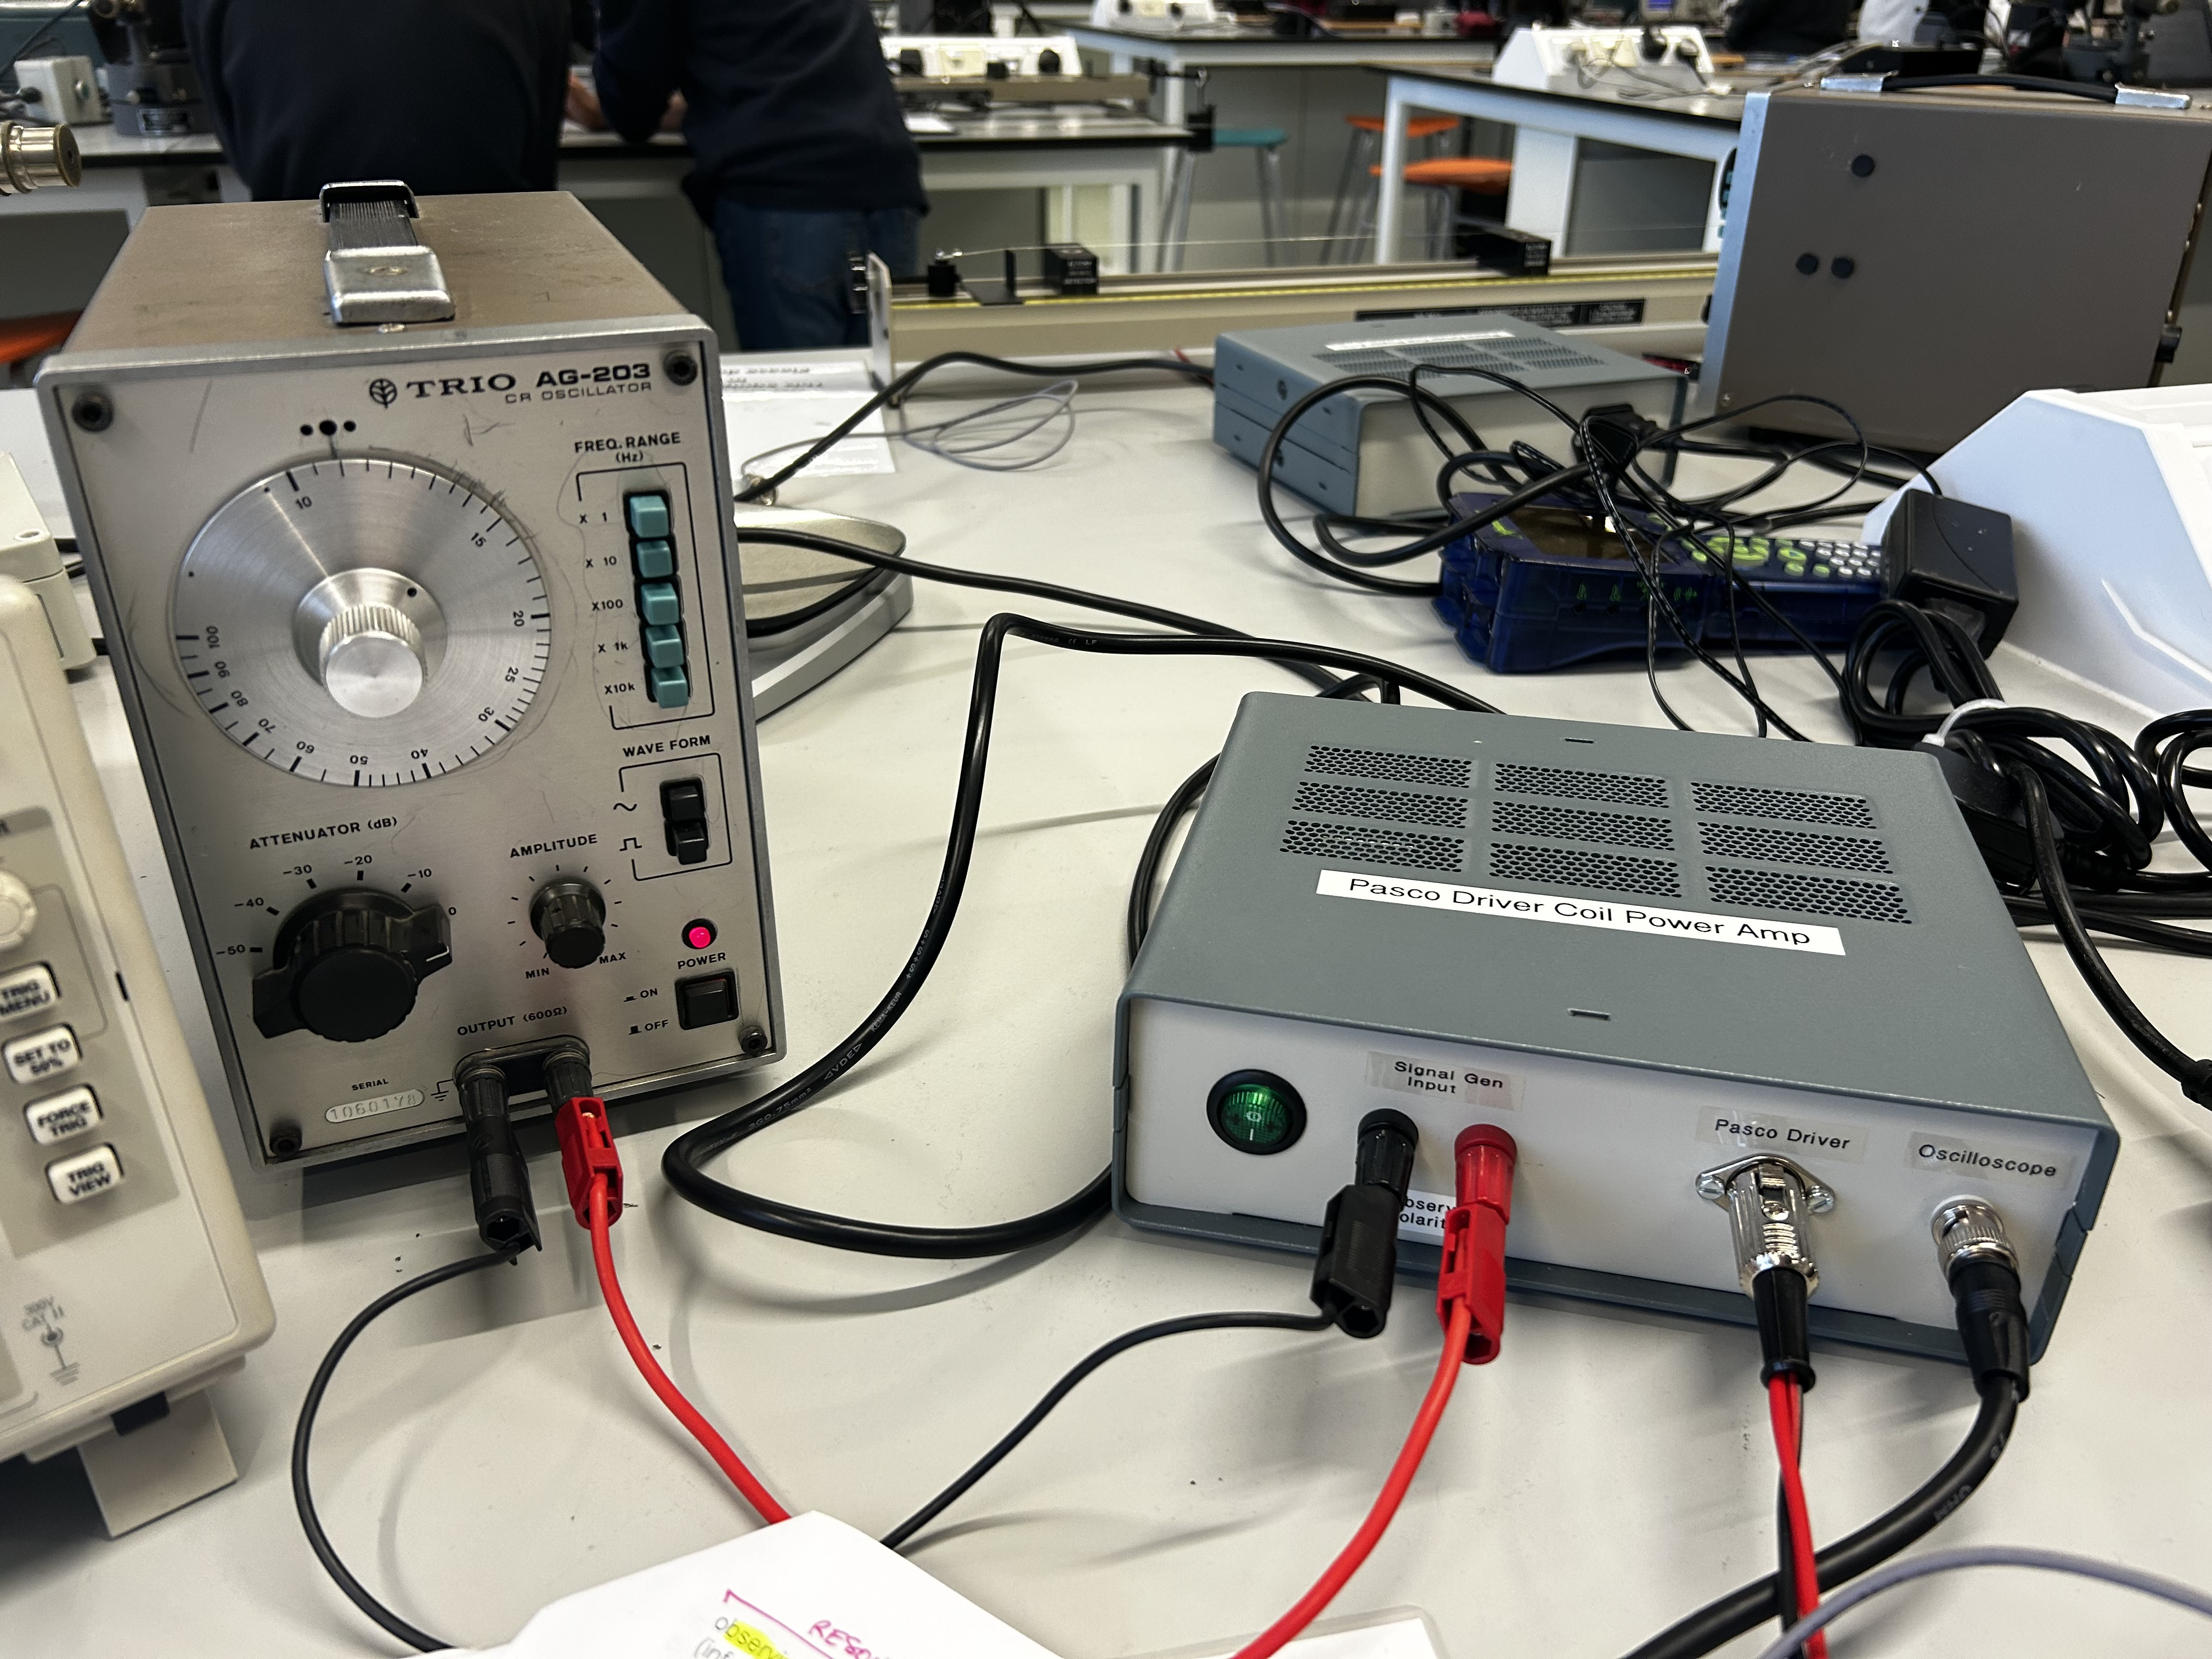
\includegraphics[width=\linewidth]{wave exp 3.jpeg}
    \captionof{figure}{\centering Image of the oscillator.}
    \label{fig:box}
\end{minipage}

The tension in the string was measured using the below formula for both parts of the experiment:

\vspace{-1.5ex}
\begin{gather}
    T = sMgz
\end{gather}

Where \textbf{s} is the slot number, \textbf{M} is the mass, \textbf{g} is the acceleration due to gravity, and \textbf{z} was the constant $0.26$.
From there, the lowest frequency at which resonance (maximum vibrations occur) was found for each varied value and recorded to be plotted in a graph.

\subsection{Varying Length Method}

For this section of the experiment the length of the string that oscillates was adjusted with teh driver and detector coil bridges as seen in figure \ref{fig:appillust}.
The length of this string was then measured with the meter stick on the apparatus, as seen in figure \ref{fig:exp}.

The slot of the weight on the tensioning level was set and left at 3, removing it as a variable for this section of the experiment.

\subsection{Varying Tension Method}

For this section of the experiment the tension of the string was varied by adjusting the slot at which the weight hung from as seen in figure \ref{fig:appillust}.

The length of the string was kept at 60 cm to remove it as a variable from the calculations.

\section{Results and Calculations} \label{sec:3}

\subsection{Application of Theory Questions}

\textit{\textbf{Q1.} A string on a guitar is 1 m long and held under a tension of 100 N. If the string has a mass of 10 g, what is the velocity of a wave on the string?}

\vspace{-1.5ex}
\begin{gather*}
    \mu = \frac{m}{L} = \frac{10 \times 10^{-3}}{1} = 10 \times 10^{-3} \text{ kg m}^{-1}
\end{gather*}
\begin{gather*}
    \implies \quad v = \sqrt{\frac{T}{\mu}} = \sqrt{\frac{100}{10 \times 10^{-3}}} = \mathbf{100 \textbf{ m s}^{-1}}
\end{gather*}

\textit{\textbf{Q2.} If a wave with a frequency of 50 Hz is sent into the string, what will its wavelength be?}

\vspace{-1.5ex}
\begin{gather*}
    v = f \lambda \quad \implies \quad \lambda = \frac{v}{f} = \frac{100}{50} = \mathbf{2} \textbf{m}
\end{gather*}

\textit{\textbf{Q3.} What is the lowest resonant frequency (the fundamental) of the bass guitar string referred to above?}

\vspace{-1.5ex}
\begin{gather*}
    \lambda_{1} = \frac{2(1)}{1} = \mathbf{2} \textbf{m} \qquad\qquad n = 1 \:\: (\text{fundamental}) 
\end{gather*}

\textit{\textbf{Q4.} What happens if a wave with a frequency which is the same as the resonant frequency enters the string?}

The string will resonate in its first (fundamental) harmonic (see §\ref{sec:1.2.2}).

\textit{\textbf{Q5.} What happens if a wave with a frequency which is different to the resonant frequency enters the string?}

No standing wave will be formed, and thus the reflection of the wave will result in little to no resonance in the string. No nodes or anti-nodes will be formed or visible as the energy is dissipated rather than amplified.

\subsection{Varying Length} \label{sec:3.2}

The mass per unit length of the wire ($\mu$) is given to be \textbf{0.39 g/m}, which is \textbf{0.00039 kg/m}.
The weight was set to slot 3, so with a weight of \textbf{0.9970 kg} the tension on the string was found to be:

\vspace{-1.5ex}
\begin{gather*}
    T = sMgz \: , \: W = mg \quad \implies \quad T = (3)(0.9970)(0.26) = \mathbf{0.77766 \textbf{N}}
\end{gather*}

The values were then inserted into a table (table \ref{tab:1}) and plotted on a graph (figure \ref{fig:lengthgraph}). The error on the metre stick is half a millimetre ($\pm 0.0005$ m) as the
length values were taken in centimetres (and converted into metres for the table and graph) and the error on the frequency is observationally estimated to be $\pm 0.05$ Hz.

The error propagation for each value was calculated with the code found in the Appendix (see §\ref{sec:A}).

\begin{minipage}{0.45\textwidth}
    \captionsetup{hypcap=false}
\begin{table}[H]
    \centering
    \begin{tabular}{|c|c|c|}
    \hline
    \textbf{L (m)} & \textbf{$\mathbf{F_{res}}$ (Hz)} & \textbf{1/L (m$\mathbf{^{-1}}$)} \\ \hline
    0.50 & 111.888 & 2.000 $\pm$ 0.0020 \\ \hline
    0.45 & 111.973 & 2.222 $\pm$ 0.0025 \\ \hline
    0.40 & 112.033 & 2.500 $\pm$ 0.0031 \\ \hline
    0.35 & 112.002 & 2.857 $\pm$ 0.0041 \\ \hline
    0.30 & 112.004 & 3.333 $\pm$ 0.0056 \\ \hline
    0.25 & 112.129 & 4.000 $\pm$ 0.0080 \\ \hline
    0.20 & 112.075 & 5.000 $\pm$ 0.0125 \\ \hline
    0.15 & 112.060 & 6.667 $\pm$ 0.0222 \\ \hline
    \end{tabular}
    \caption{\centering Table of the data gathered for the resonant frequency while varying the lenght of the string.}
    \label{tab:1}
\end{table}
\end{minipage}
\hfill
\begin{minipage}{.5\textwidth}
    \captionsetup{hypcap=false}
    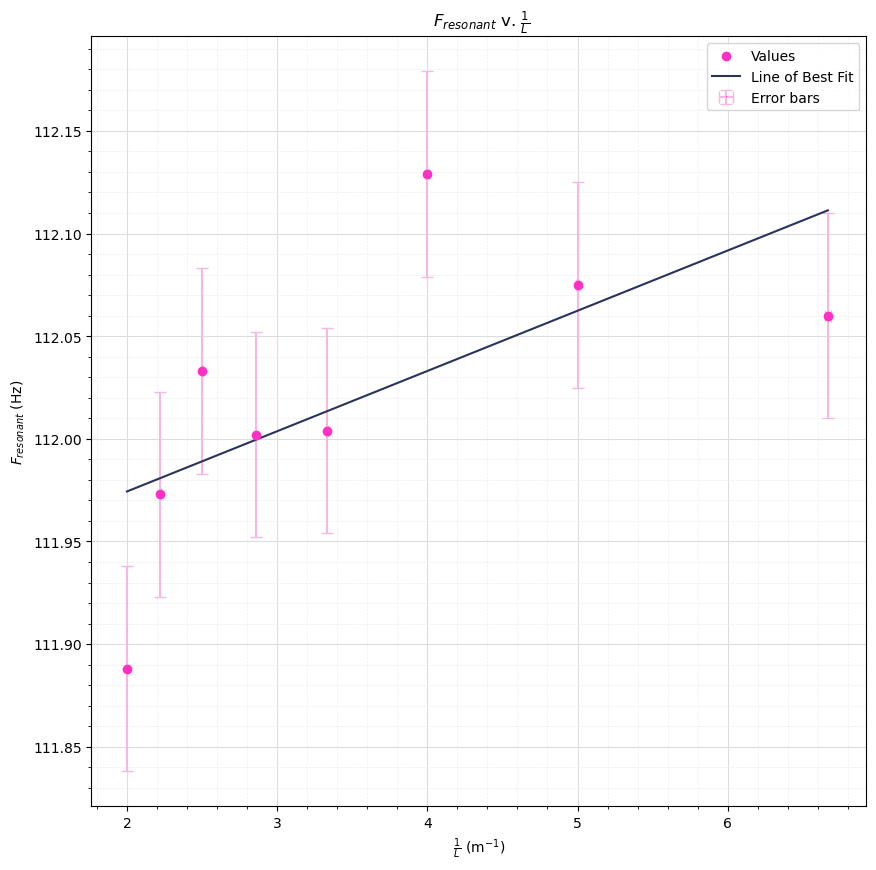
\includegraphics[width=\linewidth]{waves length graph.png}
    \captionof{figure}{\centering Graph of the data found from table \ref{tab:1}.}
    \label{fig:lengthgraph}
\end{minipage}

The slope calculated by the code for this line of best fit is found to be \textbf{0.0294}.
However, the slope of the graph can also be manually calculated by manipulating the original equation to be of the form $y=mx+c$.

\vspace{-1.5ex}
\begin{gather*}
    f = \frac{1}{2L} \sqrt{\frac{T}{\mu}} \quad \implies \quad f = \frac{1}{2} \sqrt{\frac{T}{\mu}} \cdot \frac{1}{L}
\end{gather*}

With $y = f$ and $x = \dfrac{1}{L}$ then the slope must be $m = \dfrac{1}{2} \sqrt{\dfrac{T}{\mu}}$. Plugging in the values for $\mu$ and T the slope is found to be 0.0448. The error on this value cannot be calculated
as the error on the mass per unit length $\mu$ has not been provided for the following formula:

\vspace{-1.5ex}
\begin{gather*}
    \Delta m = m \cdot \frac{1}{2} \sqrt{\left( \frac{\Delta \mu}{\mu} \right)^2 + \left( \frac{\Delta T}{T} \right)^2}
\end{gather*}

However, the percentage difference between both the theoretical (\textbf{22.327}) and calculated (\textbf{0.0294}) slope is found to be \textbf{199.47\%}. This is a very, \textit{very} significant difference.

\subsection{Varying Tension} \label{sec:3.3}

The value for the length of the string was kept constant at 0.60 m. The collected and calculated values for the tension and resonant frequencies were put into a table (table \ref{tab:2}) and plotted on a graph (figure \ref{fig:tensiongraph}).
The error on the weight was $\pm$ 0.00005 kg, and the error on the frequency was observationally estimated to be $\pm$ 1 Hz, and the error propagation for both the tensions and squared frequencies were calculated using the code found in the Appendix (see §\ref{sec:A}).

\begin{minipage}{.45\textwidth}
    \captionsetup{hypcap=false}
\begin{table}[H]
    \centering
    \begin{tabular}{|c|c|c|}
    \hline
    \textbf{T (N)}                                          & \textbf{$\mathbf{F_{res}}$ (Hz)} & \textbf{$\mathbf{F_{res}^2}$ (s$\mathbf{^{-2}}$)}            \\ \hline
    \begin{tabular}[c]{@{}c@{}}0.2592\\ $\pm$ $1.3 \times 10^{-5}$ \end{tabular} & 62.676                           & \begin{tabular}[c]{@{}c@{}}3 928.281\\ $\pm$ 125.352 \end{tabular}  \\ \hline
    \begin{tabular}[c]{@{}c@{}}0.5184\\ $\pm$ $2.6 \times 10^{-5}$ \end{tabular} & 85.081                           & \begin{tabular}[c]{@{}c@{}}7 238.777\\ $\pm$ 170.162 \end{tabular}  \\ \hline
    \begin{tabular}[c]{@{}c@{}}0.7776\\ $\pm$ $3.9 \times 10^{-5}$ \end{tabular} & 104.979                          & \begin{tabular}[c]{@{}c@{}}11 020.590\\ $\pm$ 209.958 \end{tabular} \\ \hline
    \begin{tabular}[c]{@{}c@{}}1.0369\\ $\pm$ $5.2 \times 10^{-5}$ \end{tabular} & 120.806                          & \begin{tabular}[c]{@{}c@{}}14 594.090\\ $\pm$ 241.612 \end{tabular} \\ \hline
    \begin{tabular}[c]{@{}c@{}}1.2961\\ $\pm$ $6.5 \times 10^{-5}$ \end{tabular} & 133.430                          & \begin{tabular}[c]{@{}c@{}}17 803.565\\ $\pm$ 266.680 \end{tabular} \\ \hline
    \end{tabular}
    \caption{\centering Table of the data gathered for the resonant frequency while varying the tension on the string.}
    \label{tab:2}
\end{table}
\end{minipage}
\hfill
\begin{minipage}{.5\textwidth}
    \captionsetup{hypcap=false}
    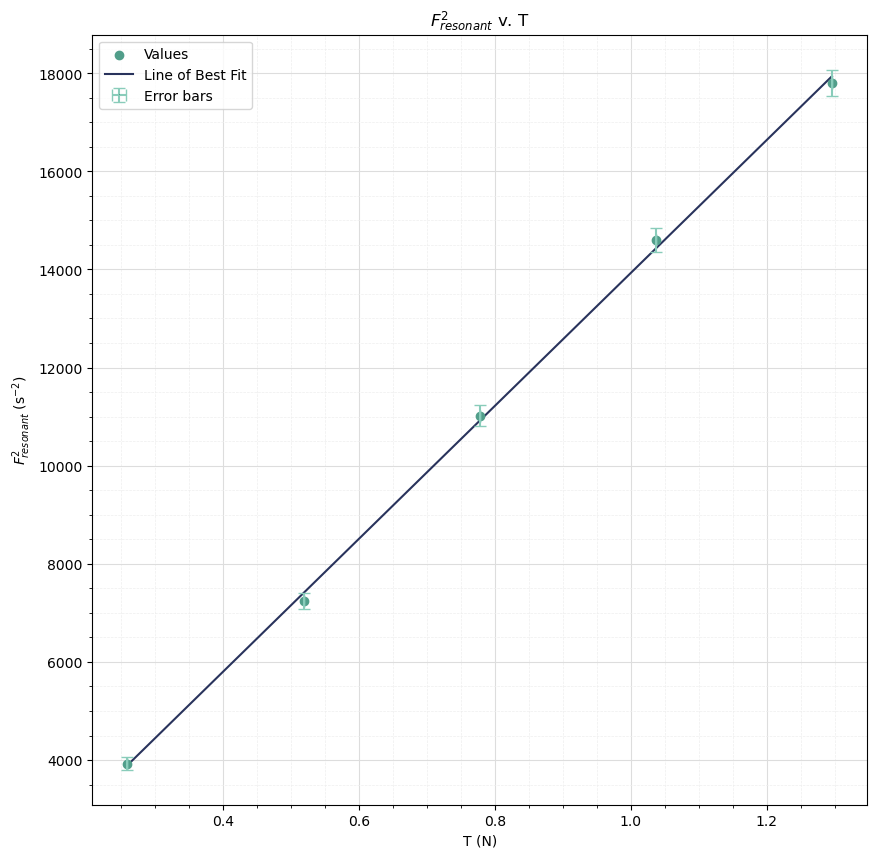
\includegraphics[width=\linewidth]{waves tension graph.png}
    \captionof{figure}{\centering Graph of the data found from table \ref{tab:2}.}
    \label{fig:tensiongraph}
\end{minipage}

The slope calculated by the code for the line of best fit is found to be \textbf{13 542.891}.
However, the slope of the graph can also be manually calculated by manipulating the original equation to be of the form $y=mx+c$:

\vspace{-1.5ex}
\begin{gather*}
    f = \frac{1}{2L} \sqrt{\frac{T}{\mu}} \quad \implies \quad f^2 = \frac{1}{4L^2} \left( \frac{T}{\mu} \right) \quad \implies \quad f^2 = \frac{1}{4L^2 \mu} T
\end{gather*}

With $y = f^2$ and $x = T$ then the slope must be $m = \frac{1}{4L^2 \mu}$. Plugging in the values for $\mu$ and L the slope is found to be 1 780.627. The error on this value cannot be calculated
as the error on the mass per unit length $\mu$ has not been provided for the following formula:

\vspace{-1.5ex}
\begin{gather*}
    \Delta m = m \cdot \frac{1}{2} \sqrt{\left( \frac{\Delta \mu}{\mu} \right)^2 + \left( \frac{2 \Delta L}{L} \right)^2}
\end{gather*}

However, the percentage difference between both the theoretical (\textbf{1 780.627}) and calculated (\textbf{13 542.891}) slope is found to be \textbf{153.52\%}. This is a \textit{very} significant difference.

Due to time constraints, the last part of this experiment was not able to be done. However, comparing to Lian Fernandes' lab report (fellow student in PHYC20080), it can be devised
that the harmonics on the string at different tensions is roughly double the previous and that the values found for this report were actually the second harmonics and not the first (fundamental)
harmonics (comparing Lian's value of \textbf{32.3 Hz} and this lab report's value of \textbf{62.7 Hz}).

\vspace{2cm}

\section{Conclusion} \label{sec:4}

While the plots accurately displayed the relationship between frequency and length/tension, the percentage discrepancies between the theoretical and experimentally-measured values is too great to ignore,
with \textbf{199.47\%} for the inverse length relationship and \textbf{153.52\%} for the tension relationship.
The theoretical values obtained by re-arranging equation \ref{eq:5} were \textbf{22.327} and \textbf{1 780.627} for the inverse length and tension relationships respectively, while the value of the straight line fit slopes
were calculated to be \textbf{0.0294} for the inverse length and \textbf{13 542.891} for the tension, yet the graphs obeyed the expected results for the line of best fit.

The arise in errors could likely be from faulty equipment as well as misunderstanding which exactly was the lowest frequency at which the string vibrated in resonance. Frequency readings are the most likely
to be of fault as that was the only factor being varied and read by machines, the oscillator and oscilloscope respectively. As can be seen in figure \ref{fig:oscil}, the string was indeed oscillating in resonance, but there is a chance
that this was not the first harmonic/fundamental frequency, which would lead to the calculations and therefore theoretical assumptions to be incorrectly based.
The provided mass per unit length could have also likely been incorrect as no error on that measurement was provided and there is no way of knowing what wire was measured to provide such a value.
In the future, individual readings of the mass per unit length of the wire could be taken during the lab at various points on the wire and averaged to account for any imperfections that could affect resonance.
The lack of a fine tuning dial on the oscillator also allowed for the possibility of discrepancies in the readings of the frequency being put across the wire, lack of precision leading to greater propagation of errors
throughout the graph.

\newpage

\section{Applications of Resonant Frequency}

\subsection{Electrical Resonance}

Information and citations sourced directly from one of my previous lab reports as information applies here \cite{meUCDlcr}.

\subsubsection{Radios Transmissions and TV Broadcasts}

Radios make use of frequency resonance to tune into broadcasts operating at specific frequencies on analogue radios, which can be heard once the the elements of the resonant circuit are in equilibrium
\cite{radio}. 
If the peak of the frequency band is too sharp some information, like high frequencies, may be lost
\cite{UCDlcr}.

\subsubsection{Environmental Monitoring}

Resonant circuits can be used in \textbf{temperature monitoring}, in which variations in \break temperature effect changes in the inductance and capacitance sensor, thereby changing the resonant frequency.
The same principle is used in \textbf{humidity monitoring}, where increases in permittivity and conductivity (proportional to humidity) leads to decreases in sensor resonant 
frequency.
This can then be expanded upon to determine \textbf{complex permittivity}, and in turn \textbf{biological growth monitoring} by measuring the changes in complex permittivity.
As humidity and temperature are bases for bacterial culture growth, changes in the Q-factor and resonant frequency can be used to monitor these developments.
Additionally, changes in the resonant frequency can also be used for \textbf{pressure monitoring} as increases in pressure are directly proportional to changes in temperature ($P \propto T$) (and, in turn, humidity).
More information with graphical and mathematical justification can be found at source \cite{ONG200133}.

\newpage

%%%%%%%%%%%%%%%%%%%%%%%%%%%%%%%%%%%

\bibliographystyle{IEEEtran}
\bibliography{References} \label{sec:ref}

\vspace{1.5cm}

\listoffigures

\listoftables

\section*{Appendix} \label{sec:A}
\addcontentsline{toc}{section}{Appendix}

\subsection*{Code}
\addcontentsline{toc}{subsection}{Code}

%

\begin{minipage}{\linewidth}
\captionsetup{hypcap=false}

\begin{mintedbox}
\begin{minted}[fontsize=\small, breaklines, baselinestretch=1.2, xleftmargin=0.5cm]{python}
import numpy as np
import matplotlib.pyplot as plt

# frequency^2 v Tension
f = np.array([62.676, 85.081, 104.979, 120.806, 133.430])
f2 = f**2
s = np.array([1,2,3,4,5])
T = 0.26 * 0.9970 * s

# frequency v 1/length
l = np.array([50, 45, 40, 35, 30, 25, 20, 15]) * 1e-2
invl = 1/l
fres = np.array([111.888, 111.973, 112.033, 112.002, 112.004, 112.129, 112.075, 112.060])

# Error propagation
errinvl = 0.0005/(l**2) # delta 1/L / 1/L = delta L / L
errT = s * 0.26 * 0.00005 # delta T = sz * delta W
errf2 = 2 * f * 1 # y = f^2 -> delta y = |d/df f^2| * delta f

print(f2, T)
print(invl, fres)

print(errinvl, errT, errf2)

\end{minted}
\end{mintedbox}
    \captionof{figure}{\centering Code used for the calculations in sections §\ref{sec:3.2} and §\ref{sec:3.3}.}
\end{minipage}


\begin{minipage}{\linewidth}
\captionsetup{hypcap=false}

\begin{mintedbox}
\begin{minted}[fontsize=\small, breaklines, baselinestretch=1.2, xleftmargin=0.5cm]{python}
slope, intercept = np.polyfit(invl, fres,1)

plt.figure(figsize=(10,10))

# Plot
plt.scatter(invl, fres, color="#ff30c4", label="Values", zorder=5)

# Error
plt.errorbar(invl, fres, xerr=errinvl, yerr=0.05, fmt=",", ecolor="#f5b8e3", color="#ff30c4", capsize=4, barsabove=True, zorder=3, label="Error bars")

#Grid
plt.minorticks_on()
plt.grid(True, which="major", linewidth=0.8, color="#DDDDDD")
plt.grid(True, which="minor", linewidth=0.5, color="#EEEEEE", linestyle="--")

#Line of Best Fit
plt.plot(np.unique(invl), np.poly1d(np.polyfit(invl, fres, 1))(np.unique(invl)), color = "#29335C", label="Line of Best Fit", zorder=4)

# Labels
plt.title(r" $F_{resonant}$ v. $\frac{1}{L}$")
plt.ylabel(r"$F_{resonant}$ (Hz)")
plt.xlabel(r"$\frac{1}{L}$ $(\text{m}^{-1})$")
plt.legend()

plt.show()

print(np.abs(slope))

\end{minted}
\end{mintedbox}
\captionof{figure}{\centering Code used for the graph in section §\ref{sec:3.2}.}
\end{minipage}
    

\begin{minipage}{\linewidth}
\captionsetup{hypcap=false}

\begin{mintedbox}
\begin{minted}[fontsize=\small, breaklines, baselinestretch=1.2, xleftmargin=0.5cm]{python}
slope, intercept = np.polyfit(T, f2, 1)

plt.figure(figsize=(10,10))

# Plot
plt.scatter(T, f2, color="#519E8A", label="Values", zorder=4)

# Error
plt.errorbar(T, f2, xerr=errT, yerr=errf2, fmt=",", ecolor="#89ccba", color="#519E8A", capsize=4, barsabove=True, zorder=5, label="Error bars")

#Grid
plt.minorticks_on()
plt.grid(True, which="major", linewidth=0.8, color="#DDDDDD")
plt.grid(True, which="minor", linewidth=0.5, color="#EEEEEE", linestyle="--")

#Line of Best Fit
plt.plot(np.unique(T), np.poly1d(np.polyfit(T, f2, 1))(np.unique(T)), color = "#29335C", label="Line of Best Fit", zorder=3)

# Labels
plt.title(r"$F_{resonant}^2$ v. T")
plt.ylabel(r"$F_{resonant}^2$ (s$^{-2}$)")
plt.xlabel("T (N)")
plt.legend()

plt.show()

print(np.abs(slope))

\end{minted}
\end{mintedbox}
    \captionof{figure}{\centering Code used for the graph in section §\ref{sec:3.3}.}
\end{minipage}
    



\end{document}